\documentclass{ctexart}
\usepackage{EC}
\begin{document}
\section{碳及其化合物}
\subsection{单质碳}
\subsubsection{石墨}
\paragraph{石墨的结构,性质与反应}
众所周知,石墨具有六边形\ce{\{C6\}}环稠合的二维层状结构.
\chemfig{graphite-1}{1}{石墨的二维层状结构示意图}
根据层间重叠方式的不同,石墨有两种异构体,即六方$\alpha$-石墨和三方$\beta$-石墨,前者在自然界中占据主要(约$70\%$).两者的晶体结构如下所示.
\bichemfig{alpha-graphite}{1}{六方$\alpha$-石墨的晶体结构示意图}{beta-graphite}{1}{三方$\beta$-石墨的晶体结构示意图}{石墨的两种异构体(黑点表示碳原子,虚线表示晶胞边界)}
从密堆积的角度描述这两种石墨的结构,六方$\alpha$-石墨的堆积层可以表示为$\cdots AB\overline{AB}AB\cdots$,而三方$\beta$-石墨的堆积层可以表示为$\cdots ABC\overline{ABC}ABC\cdots$.研磨$\alpha$-石墨可以使其转化为$\beta$-石墨,而加热$\beta$-石墨可以使其转化为$\alpha$-石墨.不完全的转化将得到湍层石墨,其中各层的堆积次序是随机的.\\
\indent 由于每一层均可以视作无限稠合的芳环,因而电子在层内是高度离域的,这使得石墨具有良好的导电性能,并且平行于层方向的电导率大约是垂直于层方向的$10^3$倍.\\
\indent 石墨的层间间距较大,只有不强的范德华力作用,使得其容易沿层平面滑动解理\footnote{\tbf{解理}(cleavage)又称\tbf{劈理},是矿物学和宝石学的常见术语,指的是矿物或宝石晶体在外力的作用下,沿一定的结晶学方向裂开成光滑平面的性质.这些光滑平面被称为\tbf{解理面}或\tbf{劈理面}.}.因此,石墨的硬度很低.\\
\indent 石墨的独特的层状结构使得它与\ce{F2}反应时控制条件就能形成理想化学式为\ce{CF}的分子.这种分子由无限延伸的椅式六元环稠合而成,所有\ce{F}原子分居平面两侧.
\paragraph{石墨的分布,生产与用途}
晶状的石墨广泛分布于全世界,然而大多数以薄片的形式存在于硅酸盐矿石中,几乎没有经济价值.由于缺乏天然的来源,石墨在工业上主要通过焦炭与二氧化硅的反应制备:
\begin{center}
    \ce{SiO2 + 3C -> SiC}\\
    \ce{SiC(s) ->T[$2500\tc$] Si(g) + C(s,\text{石墨})}
\end{center}
石墨的主要用途如下:
\begin{enumerate}[label=\tbf{\arabic*.},topsep=0pt,parsep=0pt,itemsep=0pt,partopsep=0pt]
    \item \tbf{作为铅芯的主要成分制造铅笔}\\
        石墨的层状结构易剥落,可用于纸上书写.现代铅笔笔芯以石墨和黏土制造,石墨含量越高,铅芯越软,颜色越黑.\\
        铅笔之名源自其早期雏形为铅金属所制造,而后则又因欧洲中世纪时石墨被误以为是铅的一种,而有了\tbf{黑铅}这个名称,因此铅笔一词在各语言中流传使用而未修正.中国古代的铅笔事实上确为铅粉所制,并没有石墨.
    \item \tbf{惰性电极材料}\\
        石墨的优良的导电性和稳定性使得其可以作为电极材料.这一方案显然比铂电极更加便宜,并且不会受到卤素的侵蚀.因此,电解\ce{NaCl}水溶液制备\ce{Cl2}和\ce{NaOH}时通常采用石墨电极.
    \item \tbf{核反应堆的中子减速剂}
        石墨可以有效地减缓核反应堆里中子的速度,有效控制反应进行.石墨耐高温,纯度高,是迄今为止核反应堆中极为重要的原材料.
\end{enumerate}
\subsubsection{金刚石与蓝丝黛尔石}
\paragraph{金刚石的结构与性质}
在金刚石中,\ce{C}原子以$\text{sp}^3$杂化形式与相邻的\ce{C}原子成键,从而形成无限延伸的三维结构.金刚石也有两种异构体.大多数天然得到的或人工合成的金刚石均属立方晶系,因此一般而言我们所称的金刚石为立方金刚石.1967年在美国亚利桑那州的巴林杰陨石坑第一次鉴别出了六方金刚石,并以爱尔兰晶体学家D. K. Lonsdale\footnote{1929年, D. K. Lonsdale首次利用X射线衍射法证明了苯是平面的.1931年,她又首次利用Fourier变换光谱分析法解析了六氯苯的结构,为推动芳香性的研究做出了重大贡献.她是英国皇家化学会首次选入的两个女会士之一,伦敦学院大学的首位终身女教授,国际晶体学会第一位女主席,英国科学促迸学会首位女主席.}命名为蓝丝黛尔石.两者的结构如下所示.
\bichemfig{diamond-1}{0.1}{立方金刚石的晶体结构}{diamond-2}{0.1}{六方金刚石的晶体结构}{两种金刚石的晶体结构}
事实上,分别将闪锌矿和纤锌矿中的所有原子替换为碳原子即可分别得到立方金刚石和六方金刚石.\\
\indent 蓝丝黛尔石推测为流星上的石墨坠入地球时在高温高压下形成.它保留了石墨的平行六边形结构,但层间的碳原子成键.蓝丝黛尔石相较立方金刚石不稳定,这可能是因为其中存在船式六元环(即存在重叠式构象的碳原子)所致.有研究表明,蓝丝黛尔石具有比立方金刚石更高的硬度和更强的抗压能力.然而,天然存在的蓝丝黛尔石不纯,且并不完全为六方结构.\\
\indent 金刚石是已知硬度最高的天然物质.同时,它的化学性质也非常稳定,即使在纯\ce{O2}中也要加热到$720\tc$才能燃烧.
\paragraph{金刚石的合成与应用}
由于金刚石的硬度极高且导热性极高,因此常用于用于钻探,研磨工具之上,可以用来切削和刻划其他物质.自1955年通用电气发明通过高温高压处理石墨获得人造金刚石的技术以来,人们已经可以利用气相沉积法等制成金刚石微粒,因此现在细小颗粒的人工合成钻石已经较同级天然钻石便宜.故此,天然钻石的工业价值已经完全消失,目前的主要用途已仅限于首饰与观赏.随着人工合成技术的成熟,合成钻石也进入了首饰市场,但总是遭到天然钻石公司的诋毁.
\subsubsection{石墨烯}
\paragraph{石墨烯的结构与性质}
石墨烯又称单层石墨,碳单层,是由石墨剥层制造出的碳单质.石墨烯的碳原子以$\text{sp}2$杂化轨道组成六角型呈蜂巢晶格的单层平面薄膜,其厚度仅相当于1个碳原子的直径.\\
\indent 石墨烯几乎是完全透明的,它的透光率为$97.7\%$.与石墨类似的,它具有极高的导热和导电性能.
\paragraph{石墨烯的制备与应用}
2004年,曼彻斯特大学和俄国切尔诺戈洛夫卡微电子工艺研究所的两组物理团队共同合作,首先分离出单独石墨烯平面.海姆和团队成员偶然地发现了一种简单易行的制备石墨烯的新方法,他们将石墨片放置在塑料胶带中,折叠胶带粘住石墨薄片的两侧.撕开胶带,薄片也随之一分为二.不断重复这一过程,就可以得到越来越薄的石墨薄片,而其中部分样品仅由一层碳原子构成,这就制得了石墨烯.\\
\indent 除此之外,还可以采用在\ce{Ni}基底上进行气相沉积法等方法.总之,由于石墨烯的广泛的潜在用途,人们仍然在对改进工艺,提高制备效率和纯度等方面进行努力.\\
\indent 石墨烯凭借其超凡的导电性,导热性,机械强度,柔韧性和透明度,在众多领域展现出革命性的应用潜力.在电子领域,它是制造超快芯片,柔性透明电极(用于可折叠屏幕和触摸屏)的理想材料;在能源领域,它能显著提升锂电池,超级电容器的充放电速度和容量,并用于高效太阳能电池;在材料领域,它用于制造更轻,更强,更耐用的复合材料和防腐,导电,导热涂层;此外,它在高灵敏度传感器,高效海水淡化膜,水处理过滤膜,生物医学(如药物递送,生物传感)以及可穿戴技术等方面也具有广阔前景,被视为推动未来科技发展的关键材料之一.
\subsubsection{石墨炔}
\subsubsection{富勒烯及其衍生物}
\paragraph{富勒烯的制备}
富勒烯又称球碳,是由纯碳原子组成的球形分子.这类分子可以通过在石墨电极间放电后形成的碳烟中分离得到,也可以在严格控制下使苯不完全燃烧,在形成的碳烟中分离得到.
\paragraph{足球烯的结构与反应}
1985年英国化学家哈罗德·沃特尔·克罗托博士和美国科学家理查德·斯莫利在莱斯大学制备出了第一种富勒烯,即\tbf{足球烯}\ce{C_60}.它的骨架结构与足球一致,属于$I_{\text h}$点群,具有很高的对称性,同时也是最常见和最稳定的富勒烯.
\begin{figure}[H]
    \centering
    \subfigure[\ce{C60}的结构]{
        \centering\begin{minipage}[b]{.3\linewidth}
            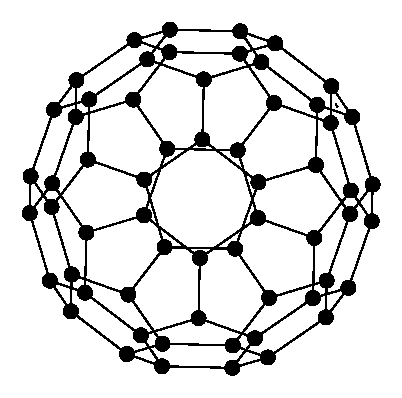
\includegraphics[scale=0.75]{picture/C60-1.eps}
        \end{minipage}
    }
    \subfigure[\ce{C60}的成键方式示意图]{
        \centering\begin{minipage}[b]{.3\linewidth}
            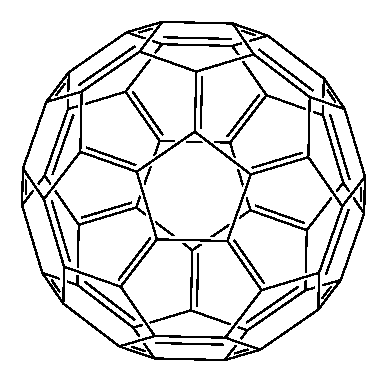
\includegraphics[scale=0.75]{picture/C60-2.eps}
        \end{minipage}
    }
    \subfigure[\ce{C60}的平面示意图]{
        \centering\begin{minipage}[b]{.3\linewidth}
            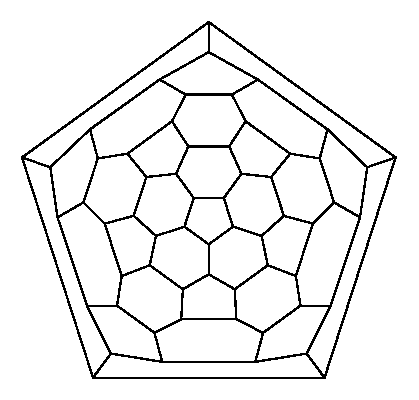
\includegraphics[scale=0.75]{picture/C60-3.eps}
        \end{minipage}
    }\vspace{-10pt}\caption{\ce{C60}分子的结构}
\end{figure}
\ce{C60}一共有12个五边形面和20个六边形面,其中每个五元环都与五个六元环相接,而每个六元环都与三个五元环和三个六元环交替相接.不难看出,\ce{C60}中的所有\ce{C}原子均等价.
\paragraph{\ce{C60}的体积}
\ce{C60}中两个六元环共用\ce{C-C}键的键长为$138.8\text{ pm}$,五元环和六元环共用\ce{C-C}键的键长为$143.2\text{ pm}$.根据键长数据,我们可以求出\ce{C60}分子的体积\footnote{当然,我们可以用内切球,外接球等方法近似计算其体积.这里采取精确计算的办法.}.\\
\indent 不难看出,\ce{C60}的结构与三角二十面体有很大的相似性.为此,我们可以把所有两个六元环共用的边延长,将\ce{C60}补全为一个正三角二十面体.这一过程的逆过程即在三角二十面体的每个顶点截去一个正五棱锥.由于原来的三角二十面体的每个面都是正三角形,因此截面的五边形的边长与五棱锥的棱长相等.因此,这个正三角二十面体的边长为
\[a=d_{66}+2d_{56}=(138.8+143.3\times2)\text{pm}=425.2\text{ pm}\]
经过三角二十面体的对棱(不妨记为$A_1A_2$和$A_3A_4$)取截面,那么$A_1A_2A_3A_4$应当是一个矩形,矩形的中心$O$即为三角二十面体的中心.短边长度$d_1=a=425.2\text{ pm}$,长边即五边形对角线,其长度
\[d_2=\sqrt{2a^2\left(1-\cos108^\circ\right)}=688.0\text{ pm}\]
于是中心$O$到顶点$A$的距离为
\[r=\dfrac{\sqrt{d_1^2+d_2^2}}{2}=404.4\text{ pm}\]
取任意三角形面的面心$B$,中心$O$到$B$的距离为
\[h_1=\sqrt{r^2-\left(\dfrac{\sqrt3}{3}a\right)^2}=321.3\text{ pm}\]
于是该三角二十面体的体积为
\[V_1=20\cdot\dfrac13\cdot\dfrac{\sqrt3}{4}a^2h_1=1.677\times10^{8}\text{ pm}^3\]
\indent 现在我们计算截去的五棱锥的体积.五棱锥的高为
\[h_2=\sqrt{d_{56}^2-\left(\dfrac{d_{56}}{2\cos54^\circ}\right)^2}=75.28\text{ pm}\]
于是五棱锥的体积为
\[V_2=\dfrac13\cdot\left(5\cdot\dfrac12\cdot d_{56}\cdot\dfrac{\tan54^\circ d_{56}}{2}\right)\cdot h_2=8.854\times10^5\text{ pm}^3\]
\indent 对于\ce{C60}而言,一共截去了$12$个五棱锥,因此\ce{C60}的体积为
\[V=V_1-12V_2=1.571\times10^{8}\text{ pm}^3\]
\indent 这是一道锻炼空间想象和立体几何能力的题目.你还可以采取其它计算方法得到它的体积.
\paragraph{\ce{C60}中碳的杂化形式}
在探讨这一问题之前,我们需要了解一些关于杂化的知识.$\text{sp}^i$杂化的轨道的波函数为
\[\psi_{\text{sp}^i}=a\phi_{\text s}+b_x\phi_{\text{p}_x}+b_y\phi_{\text{p}_y}+b_z\phi_{\text{p}_z}\]
其中$\phi_{\text s}$和$\phi_{\text{p}_x},\phi_{\text{p}_y},\phi_{\text{p}_z}$分别为$s$轨道和三个$p$轨道的波函数.为了方便考虑,我们最好让$\text{p}$轨道归一化.令
\[b=\sqrt{b_x^2+b_y^2+b_z^2}\ \ \ \ \ \phi_{p}=\dfrac{b_x\phi_{\text{p}_x}+b_y\phi_{\text{p}_y}+b_z\phi_{\text{p}_z}}{\sqrt{b_x^2+b_y^2+b_z^2}}\]
你可以将$\phi_{\text{p}_x},\phi_{\text{p}_y},\phi_{\text{p}_z}$分别视作空间中三个方向上的单位向量,上述过程实际上是求出三个$\text p$轨道线性组合后指向方向的单位向量,这就是归一化$\text p$轨道的意义.由于$\text{s}$轨道并无特殊取向,因此$\text{sp}^i$杂化的轨道取向由$\phi_p$的取向决定.\\
\indent 现在再来考虑组合后的波函数本身应当满足的性质:归一性和正交性.为了方便,下面就用向量的形式表示函数.对于轨道$\phi_{\text{sp}^i}$,归一性要求
\[a^2+b^2=1\]
现在考虑两个$\phi_{\text{sp}^i}$轨道,将它们分别表示为
\[\overrightarrow{\psi_{\text{sp}^i_A}}=a\overrightarrow{\phi_{\text{s}}}+b\overrightarrow{\phi_{\text{p}_A}}\ \ \ \ \ \overrightarrow{\psi_{\text{sp}^i_B}}=a\overrightarrow{\phi_{\text{s}}}+b\overrightarrow{\phi_{\text{p}_B}}\]
它们之间的夹角,即键角为$\theta$,这意味着决定两者方向的$p$轨道函数的夹角为$\theta$.正交性要求
\[\overrightarrow{\psi_{\text{sp}^i_A}}\cdot\overrightarrow{\psi_{\text{sp}^i_B}}=0\]
由于$s$轨道和任意方向上的$p$轨道都是正交的,于是$\overrightarrow{\phi_{\text{s}}}\cdot\overrightarrow{\phi_{\text{p}}}=0$.于是上式即为
\[a^2+b^2\overrightarrow{\phi_{\text{p}_A}}\cdot\overrightarrow{\phi_{\text{p}_B}}=0\]
我们说过,$\overrightarrow{\phi_{\text{p}}}$的几何意义为指向空间中某一方向的单位向量,那么两个夹角为$\theta$的单位向量的内积显然应当是$\cos\theta$.于是就有
\[a^2+b^2\cos\theta=0\]
将归一化条件代入其中就有
\[a^2=-\dfrac{\cos\theta}{1-\cos\theta}\ \ \ \ \ b^2=\dfrac{1}{1-\cos\theta}\]
采取$\text{sp}^i$意味着$\text{s}$轨道和$\text{p}$轨道的比例为$1:i$,这可以用线性组合系数的平方之比来表示,这样就有
\[i=\dfrac{b^2}{a^2}\]
结合上面的式子就有
\[1+i\cos\theta=0\]
或者
\[\theta=\arccos\left(-\dfrac1i\right)\]
这样,你就可以计算各种$\text{sp}^i$杂化中$i$的具体数值,例如\ce{H2O}中的\ce{O}接近$\text{sp}^4$杂化.\\
\indent 对于\ce{C60}而言,我们可以近似地采取平均键角进行计算.每一个碳都被两个六边形和一个五边形所共用,平均键角
\[\overline{\theta}=\dfrac{108^\circ+2\times120^\circ}{3}=116^\circ\]
于是杂化指数
\[i=-\dfrac{1}{\cos116^\circ}=2.28\]
这就是\ce{C60}中的\ce{C}原子采取$\text{sp}^{2.28}$杂化的由来.
\paragraph{\ce{C60}的晶体结构}
正常情况下,\ce{C60}晶体属立方晶系,\ce{C60}分子按照立方最密堆积形成晶体.\\
\indent 说到这一晶体的结构,就不得不提到\ce{K3C60}这一化合物.其中\ce{K+}填入所有\ce{C60}形成的四面体空隙和八面体空隙.这一物质的有趣的一点是其中\ce{K}的质量分数为$14.000\%$\footnote{所谓蕉下客.}.
\paragraph{\ce{C60}的化学性质}
尽管结构中大量存在苯环,\ce{C60}的芳香性却并不像苯一样如此明显.从键长数据也可以看出,\ce{C60}中的双键更多时候趋向于定域化,这意味着它能发生与烯烃类似的反应.此外,大的共轭体系也使得其能被单电子氧化/还原.以下是一些反应的例子.
\begin{enumerate}[label=\tbf{\arabic*.},topsep=0pt,parsep=0pt,itemsep=0pt,partopsep=0pt]
    \item \tbf{加成反应}\\
        \ce{C60}能被各种手段加氢.Birch还原能将其还原为\ce{C60H32},用二氢化蒽能将其还原为\ce{C60H36},等等.然而,\ce{C60H60}却因为键角的缘故而难以得到.\\
        \ce{C60}也可以与卤素反应.与\ce{F2}的反应倾向于生成$1,2$位的二取代物,而与\ce{Cl2}和\ce{Br2}的反应倾向于加成到相距较远的\ce{C}原子上,例如\ce{C60Br8}和\ce{C60Br24}.\\
        \ce{C60}也可以与\ce{PhCN2}等卡宾前体反应生成含有三元环的\ce{C61Ph2}.它也可以自己发生$[2+2]$环加成反应二聚成为\ce{C120}.
    \item \tbf{氧化/还原反应}\\
        在合适的氧化剂存在下,可以形成\ce{C60^n+};在合适的还原剂存在下则可以形成\ce{C60^n-}.
\end{enumerate}
\paragraph{其它富勒烯}
除去最常见的\ce{C60}之外,还有\ce{C70},\ce{C84}等富勒烯分子.它们也是笼状结构的分子,但对称性并没有\ce{C60}高.
\subsubsection{碳纳米管}
\subsubsection{无定形碳}
\paragraph{无定形碳的分布}
碳在史前就被认为是一种物质(炭,烟灰),而学界承认碳是一种元素却是18世纪几个实验的结论.大部分无定形碳都含有石墨的层状结构,然而晶体化程度很低,没有固定形状和周期性结构规律,同时经常掺杂很多其它元素.
\end{document}